\textcolor{ubuntu_orange}{Konta sieciowe} to specjalny program w Ubuntu, pozwalający sprząc system bezpośrednio z różnymi dostawcami usług sieciowych. Przykładowo, po dodaniu konta Google można łączyć się z czatem Google za pomocą wbudowanego programu Empathy, czy synchronizować zdjęcia z usługą Picasa za pośrednictwem programu Shotwell. Na podobnej zasadzie działa połączenie z kontem Facebooka, Flickr czy Twittera. Użycie \textcolor{ubuntu_orange}{Kont sieciowych} pozwala skorzystać z dwustopniowego uwierzytelnienia, nawet w programach, które w innych warunkach tego nie potrafią.

\begin{center}
	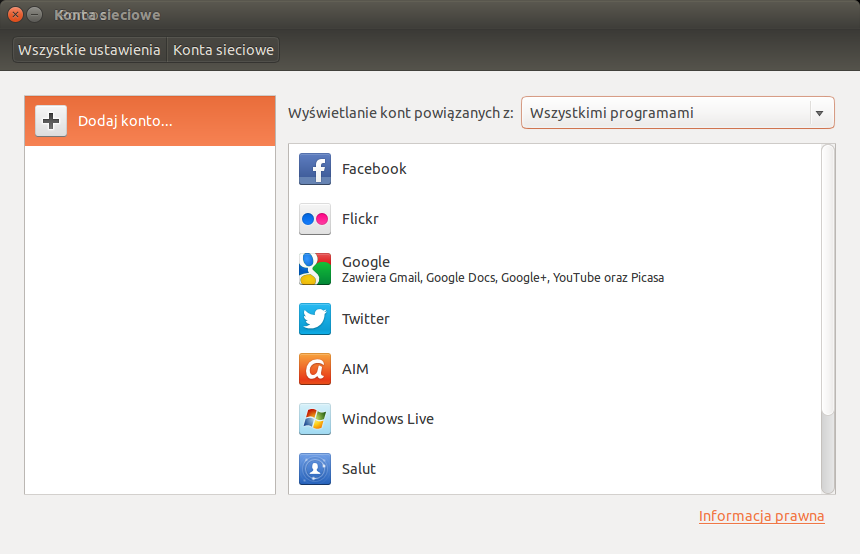
\includegraphics[width=\linewidth]{images/programy_kontaOnline1.png}
\end{center}

Aby dodać konto do systemu, wyszukaj w Dashu \textcolor{ubuntu_orange}{Konta sieciowe} i uruchom program. W otwartym oknie kliknij \textcolor{ubuntu_orange}{+ Dodaj konto} w lewym panelu, a następnie z prawego wybierz interesującego cię dostawcę. Zostaniesz teraz poproszony o uwierzytelnienie usługi w systemie.

Możesz zsynchronizować więcej niż jedną usługę. Program \textcolor{ubuntu_orange}{Konta sieciowe} pozwala ponadto zarządzać tym, jakie programy do jakich usług mają dostęp. 
